\begin{taged}{自醒}
\section{2022-05-25 酒井法子}
\end{taged}

这几天,\href{https://www.weibo.com/u/1504965390}{王心凌} 占据了网络的头条。
虽然她的《爱你》及另外的几首歌也在我的歌单里,但对我而言,她只是众多女歌手中的一员,没有特别的感觉。
只因她最火的时候,我已经不再是十来岁的少年。

我心中的女神,则是 \href{https://baike.baidu.com/item/酒井法子/265809}{酒井法子} 和 \href{https://baike.baidu.com/item/周慧敏/6702}{周慧敏}。

\begin{figure}[htbp]
    \centering
    \begin{minipage}{6cm}
        \centering
        
\includegraphics[width=6cm]{pic/酒井法子.jpg}
        \caption*{酒井法子}
    \end{minipage}
    \quad
    \begin{minipage}{10cm}
        \centering
        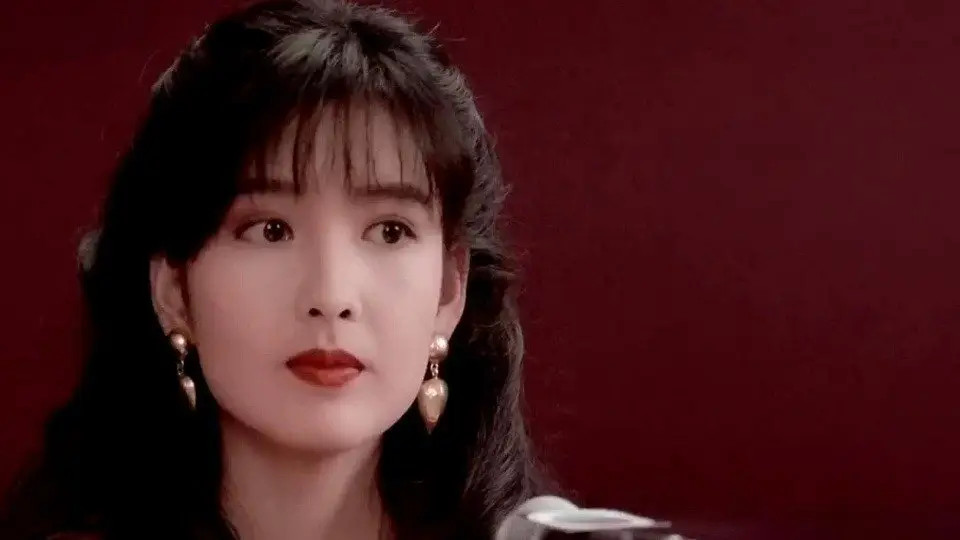
\includegraphics[width=10cm]{pic/周慧敏.jpg}
        \caption*{周慧敏}
    \end{minipage}
\end{figure}

我是在高中才首次接触到酒井法子的。
一个叫徐伟的朋友,他有酒井法子的磁带,借我听了一段时间。这一听不要紧,哇,这姑娘长得可爱,声音甜美,就她了。
后来,我自己攒了些钱,把当时能买到的法子的磁带都买了,总共大概五六盒,每盒十块钱,不便宜。如果我没有记错,高中在学校吃一顿午饭,只要七毛钱。

法子的很多歌我都听了成百上千遍:

\begin{itemize}[nosep, left=\parindent]
    \item 《碧いうさぎ (碧绿色的兔子)》
    \item 《夢冒険(梦冒险)》
    \item 《微笑みを見つけた (发现微笑)》
    \item 《あなたに天使が見える時 (当你看见天使的时候)》
    \item ……
\end{itemize}

我手机的闹钟音乐,就设置为《碧绿色的兔子》。有时午觉醒来,刻意不去关闹钟,这样又可以完整的听一遍。

